\renewcommand*{\arraystretch}{1.5}
\begin{tabularx}{15cm}{|p{2.1cm}@{\hskip 1ex}|@{\hskip 1ex}X|}
	\hline
	number      & 25                                                          \\ \hline
	title       & Weighted paths                                                           \\ \hline
	\multicolumn{2}{|c|}{ 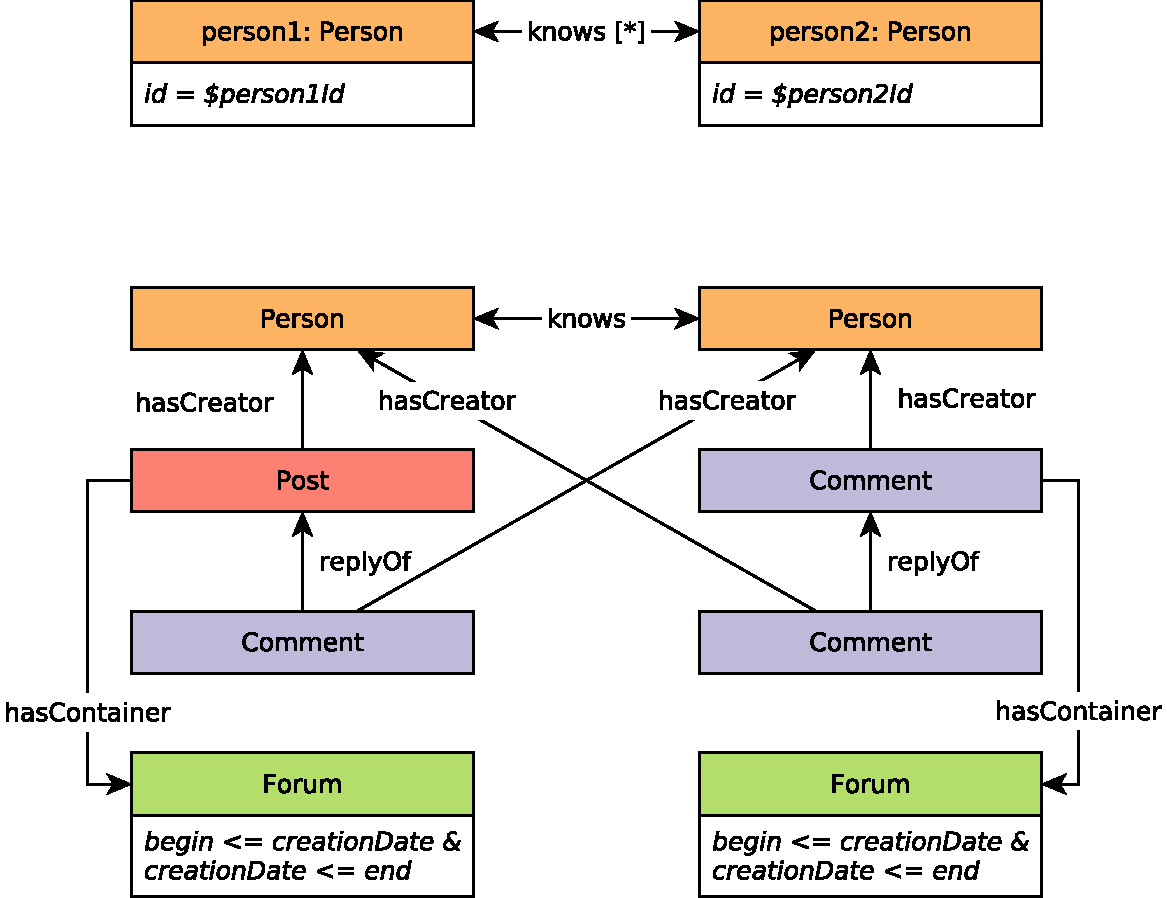
\includegraphics[scale=\patternscale,margin=0cm .2cm]{patterns/q25}} \\ \hline
	description & Given two Persons, find all (unweighted) shortest paths between these
two Persons, in the subgraph induced by the Knows relationship.

Then, for each path calculate a weight. The nodes in the path are
Persons, and the weight of a path is the sum of weights between every
pair of consecutive Person nodes in the path.

The weight for a pair of Persons is calculated such that every reply (by
one of the Persons) to a Post (by the other Person) contributes 1.0, and
every reply (by ones of the Persons) to a Comment (by the other Person)
contributes 0.5.

Only consider messages that were created in a forum that was created
within the timeframe \texttt{{[}startDate,\ endDate{]}}.

Return all the paths with shortest length, and their weights.
 \\ \hline
	
	parameters  &
	\multicolumn{1}{>{\raggedright}X|}{
		\variable{person1Id}{64bitInteger} \\
		\variable{person2Id}{64bitInteger} \\
		\variable{startDate}{Date} \\
		\variable{endDate}{Date} 
		}\\ \hline
	result      &
	\multicolumn{1}{>{\raggedright}X|}{
		\variable{person.id}{64bitInteger}Identifiers representing an ordered sequence of the Persons in the path weight
		}\\ \hline
	sort        &
	\multicolumn{1}{>{\raggedright}X|}{
		\sortentry{weight}{\desc}The order of paths with the same weight is unspecified
		}\\ \hline
	choke points        &
	\multicolumn{1}{>{\raggedright}X|}{
		\chokepoint{1.2}, 
		\chokepoint{2.1}, 
		\chokepoint{2.2}, 
		\chokepoint{2.4}, 
		\chokepoint{3.3}, 
		\chokepoint{5.1}, 
		\chokepoint{5.3}, 
		\chokepoint{7.2}, 
		\chokepoint{7.3}
		}\\ \hline
\end{tabularx}
\clearpage
